\section{Problemstellung}

Die Arbeit beschäftigt sich mit dem Problem der zeitnahen und transparenten Rückverfolgung von Chargen und Einzelprodukten über den gesamten Verlauf der Wertschöpfungskette in Produktionsnetzwerken.\\

Die wissenschaftliche Fragestellung der Arbeit lautet daher: Kann die Blockchain Technologie den Prozess der Rückverfolgung von Chargen und/oder individuellen Produkten von der Rohstoffgewinnung bis hin zum letztendlichen Verkauf an den Endverbraucher für alle Teilnehmer der Wertschöpfungskette transparenter und sicherer gestalten?\\

Dafür ist zu klären,

\begin{enumerate}
  \item ob mit der Blockchain Technologie eine Abbildung von komplexen Trenn- und Mischprozessen realisiert werden kann.
  \item Ob Informationen über Teilprozesse zusammengefasst werden können bei gleichbleibender Transparenz für andere Teilnehmer - Rezepturgeheimnisse müssen geschützt bleiben im Fall der Fleischwarenindustrie.
  \item Ob ein Blockchain System gewisse Unschärfe-/Abstraktions-Funktionen realisieren kann zum Schutz der Marktteilnehmer.
  \item Und ob eine Möglichkeit exisitert, dass auch externe Dienstleister, die Teil des Prozesses eines Teilnehmers der Lieferkette sind, mit eingebunden werden können ohne das Informationen verfälscht werden. Beispielsweise durch den Einsatz von multiplen Blockchains die untereinander wieder einen konsisten und sicheren Datenaustausch ermöglichen. (siehe Abbildung \ref{fig:multi-blockchain-example})
\end{enumerate}

\begin{figure}[h!]
	\centering
	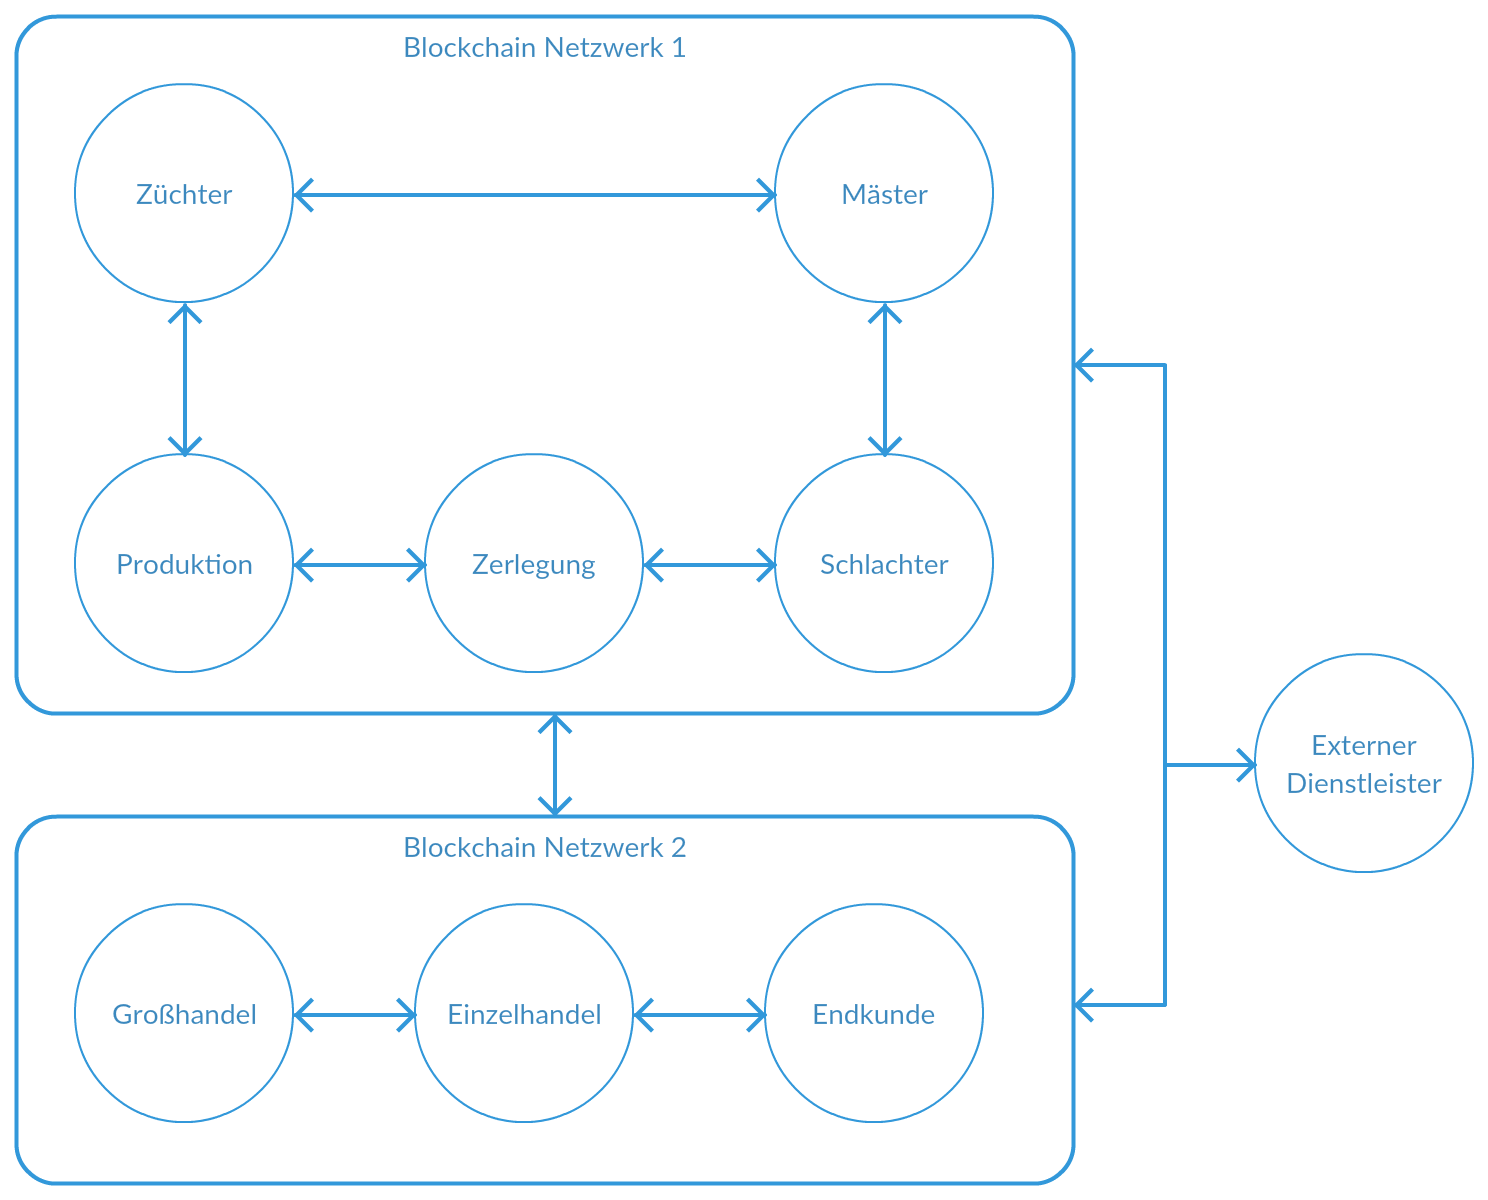
\includegraphics[width=0.8\linewidth]{pictures/Multi-Blockchain-Example}
	\caption[Multiple Blockchains innerhalb der Lieferkette]{Multiple Blockchains innerhalb der Lieferkette (eigene Darstellung)}
	\label{fig:multi-blockchain-example}
\end{figure}

%Soll die Blockchain Technologie zum Einsatz kommen gibt es offene Fragen. Eine Blockchain ist keine Silberkugel für sämtliche betriebswirtschaftliche Prozesse. Viel mehr kann eine Blockchain als Skalpell dienen um präzise ein bestimmtes Problem zu lösen.\\

%\begin{itemize}
%	\item Technologie ist so neu und frisch verfügbar im Industriekontext
%	\item Ermittlung und Definition möglicher Geschäftsprozesse der Energiewirtschaft
%	\item Vorhandene Lösungen am Markt vergleichen für den Einsatz
%	\item Mehrwert eines DLT-basierten Geschäftsprozesses herausarbeiten
%	\item Spieltheorie neue Geschäftsfelder Blockchain
%\end{itemize}

%Video [Wir und die Blockchain (The Blockchain and Us) (2017) - Deutsche Synchronfassung/German version - YouTube](\url{https://www.youtube.com/watch?v=x2mKDWsNijo})

% konkrete Beschreibung des Problems

\newpage
